% Book styling for the PDF edition. Fonts ship with TeX Live (TeX Gyre, Source Code Pro).
\usepackage{fontspec}
% Loaded by file name so the build never depends on a system font index.
\setmainfont{texgyrepagella}[Extension=.otf, UprightFont=*-regular,
  BoldFont=*-bold, ItalicFont=*-italic, BoldItalicFont=*-bolditalic]
\setsansfont{texgyreheros}[Extension=.otf, UprightFont=*-regular,
  BoldFont=*-bold, ItalicFont=*-italic, BoldItalicFont=*-bolditalic]
\setmonofont{SourceCodePro}[Extension=.otf, Scale=0.84, UprightFont=*-Regular,
  BoldFont=*-Bold, ItalicFont=*-RegularIt, BoldItalicFont=*-BoldIt]

\usepackage{xcolor}
% Cobalt & Citrus — the suite palette shared with Yesod/Pitput siblings.
% Tokens (see branding/palettes.json "cobalt"): paper, ink, signal, wire.
\definecolor{hrxpaper}{HTML}{EEF2FF}
\definecolor{hrxink}{HTML}{132548}
\definecolor{hrxsignal}{HTML}{2454D9}
\definecolor{hrxcitrus}{HTML}{D5ED42}
\definecolor{hrxcitrustext}{HTML}{445108}
\definecolor{hrxpanel}{HTML}{E2E8F7}
\definecolor{hrxmuted}{HTML}{52617B}
\definecolor{hrxline}{HTML}{BAC6DC}
\definecolor{hrxaccent}{HTML}{2454D9}
\definecolor{hrxnote}{HTML}{E2E8F7}
\definecolor{hrxnoteframe}{HTML}{2454D9}
\definecolor{hrxtip}{HTML}{F5FADB}
\definecolor{hrxtipframe}{HTML}{445108}
\definecolor{hrxwarn}{HTML}{E2E8F7}
\definecolor{hrxwarnframe}{HTML}{132548}
\definecolor{hrxside}{HTML}{E2E8F7}
\definecolor{hrxsideframe}{HTML}{52617B}

\usepackage{graphicx}
\newcommand{\BookSubtitle}{Launching, Supervising and Scaling\\AI Coding Agents}
\newcommand{\BookDeck}{A harness launcher for Codex, Claude Code and OpenCode through one model gateway}
% Edition stamp: defaults below are overridden at build time by latex/version.tex
% (generated by book/tools/build.sh from the current date and git revision).
\newcommand{\BookBuildDate}{\today}
\newcommand{\BookRevision}{dev}
\IfFileExists{latex/version.tex}{\input{latex/version.tex}}{}
\makeatletter
\renewcommand{\maketitle}{%
  \newgeometry{margin=0in}
  \begin{titlepage}
    \pagecolor{hrxink}\color{white}
    \thispagestyle{empty}
    \noindent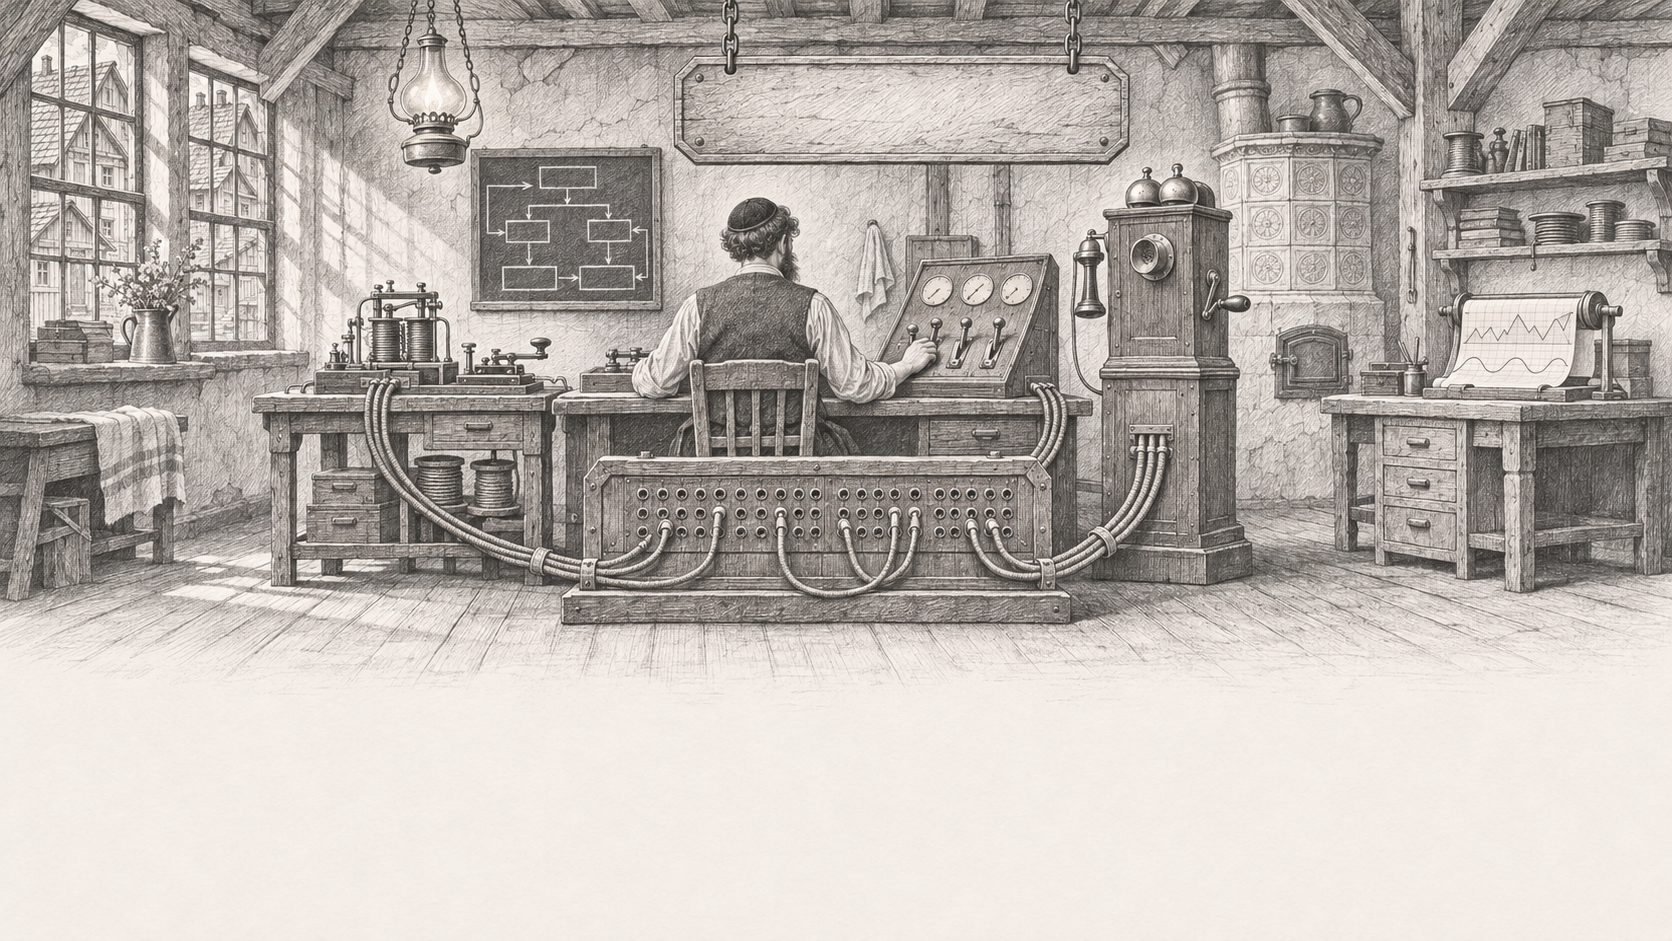
\includegraphics[width=\paperwidth]{brand/cover-art.png}\par
    \vspace{0.34in}
    \hspace*{0.62in}
\includegraphics[height=0.52in]{brand/marks/convergence-white.pdf}%
    \hspace{0.18in}\raisebox{0.06in}{\sffamily\bfseries\fontsize{30}{30}\selectfont hrx}\par
    \vspace{0.2in}
    \hspace*{0.62in}\begin{minipage}{5.76in}
      {\sffamily\bfseries\fontsize{19}{23}\selectfont \BookSubtitle\par}
      \vspace{0.16in}
      {\color{hrxcitrus}\rule{1.4in}{2.2pt}\par}
      \vspace{0.18in}
      {\sffamily\fontsize{11}{15}\selectfont\color{white!84}\BookDeck\par}
    \end{minipage}
    \vfill
    \hspace*{0.62in}\begin{minipage}{5.76in}
      {\sffamily\fontsize{10}{14}\selectfont\color{white!74}
        \BookBuildDate\par}
      \vspace{0.04in}
      {\sffamily\fontsize{8.5}{11}\selectfont\color{white!52}
        Revision \BookRevision\par}
      \vspace{0.1in}
      {\sffamily\bfseries\large Stephen Barr\par}
    \end{minipage}
    \vspace{0.5in}
  \end{titlepage}
  \restoregeometry
  \pagecolor{white}\color{black}
  \cleardoublepage
}
\makeatother

\AtBeginDocument{\hypersetup{
  pdftitle={hrx: Launching, Supervising and Scaling AI Coding Agents},
  pdfauthor={Stephen Barr},
  pdfsubject={A practical guide to hrx, a harness launcher for Codex, Claude Code and OpenCode}
}}

\usepackage[most]{tcolorbox}
\tcbset{hrxbase/.style={breakable, enhanced, boxrule=0pt, leftrule=2.5pt, arc=0pt,
  left=8pt, right=8pt, top=6pt, bottom=6pt, before skip=10pt, after skip=10pt,
  fonttitle=\sffamily\bfseries\small, coltitle=black, attach title to upper={\par\smallskip}}}
\newtcolorbox{hrxnote}[1]{hrxbase, colback=hrxnote, colframe=hrxnoteframe, title={#1}}
\newtcolorbox{hrxtip}[1]{hrxbase, colback=hrxtip, colframe=hrxtipframe, title={#1}}
\newtcolorbox{hrxwarning}[1]{hrxbase, colback=hrxwarn, colframe=hrxwarnframe, title={#1}}
\newtcolorbox{hrxsidebar}[1]{hrxbase, colback=hrxside, colframe=hrxsideframe,
  leftrule=0pt, toprule=0.6pt, bottomrule=0.6pt, title={#1}}

\usepackage{titlesec}
\titleformat{\chapter}[display]{\sffamily\bfseries\Huge}
  {\color{hrxaccent}\large\MakeUppercase{\chaptertitlename}\ \thechapter}{8pt}{}
\titleformat{\section}{\sffamily\bfseries\Large}{}{0pt}{}
\titleformat{\subsection}{\sffamily\bfseries\large}{}{0pt}{}
\titleformat{\subsubsection}{\sffamily\bfseries}{}{0pt}{}
\titleformat{\part}[display]{\sffamily\bfseries\Huge\centering}
  {\color{hrxaccent}\Large\MakeUppercase{\partname}\ \thepart}{12pt}{}

\usepackage{fancyhdr}
\pagestyle{fancy}
\fancyhf{}
\fancyhead[LE]{\sffamily\small\thepage\quad\leftmark}
\fancyhead[RO]{\sffamily\small\rightmark\quad\thepage}
\renewcommand{\headrulewidth}{0pt}
\renewcommand{\chaptermark}[1]{\markboth{#1}{}}
\renewcommand{\sectionmark}[1]{\markright{#1}}

\setlength{\parskip}{4pt plus 1pt}
\setlength{\parindent}{0pt}
\usepackage{fvextra}
\DefineVerbatimEnvironment{Highlighting}{Verbatim}{breaklines,breakanywhere,commandchars=\\\{\}}
